\section{Gradient Descent}
\subsection{Introduction}
Gradient Descent is an algorithm used to iteratively minimize functions $f: \mathbb{R}^n \to \mathbb{R}$ of multiple values.

\subsection{Directional derivatives}
Since $f$ is a function of multiple values, it does not suffice to.

From the definition of the directional derivative it follows that it evaluates to $\nabla f \cdot u$. A rigorous proof can be found in [1], but as an intuition, the change of $f(x)$ in direction $u$ can be thought of as $u_1$ times the change in $x_1$ plus $u_2$ times the change in $x_2$ plus \ldots which results in $\sum_{i=0}^{n}\frac{\partial f}{\partial x_i}u_i = \nabla f \cdot u$.

Following Goodfellow et al. [2], we can find the direction in which $f$ decreases fastest using the directional derivative:
\begin{equation*}
\begin{gathered}
\min_u \nabla f \cdot u \\
= \min_u \lVert u \rVert_2 \lVert \nabla f \rVert_2 \cos \theta
\end{gathered}
\end{equation*}
\ldots
\\\\
Our goal is to choose a $\Delta v$ that minimizes $\Delta C \approx \nabla C \cdot \Delta v$. The Cauchy--Schwarz inequality tells us that $|\nabla C \cdot \Delta v|$ is constrained by $\lVert v \rVert \lVert \nabla C \rVert$ where $|\nabla C \cdot \Delta v| = \lVert v \rVert \lVert \nabla C \rVert$ if and only if $\Delta v = \eta \nabla C$.
Since $\nabla C \cdot \eta \nabla C = \eta \lVert \nabla C \rVert^2 > 0$ we can choose $\Delta v = -\eta \nabla C$ to minimize $\Delta C$.

Gradient Descent can further be extended to include the momentum of the function \cite{DBLP:journals/corr/Ruder16}.

Following \cite{Goodfellow-et-al-2016}, one can represent neural networks as a directed cyclical graph.

Hornik\cite{DBLP:journals/nn/Hornik91} has shown that.


\begin{figure}
	\begin{center}
		% !TeX root = dm-template.tex

\begin{tikzpicture}[scale=.8]
	\begin{axis}[axis lines = left,xlabel = $x$, ylabel = {$\sigma(x)$},]
		\addplot [domain=-8:8, samples=200, color=red, style=semithick]
		{1/(1+exp(-x))};
	\end{axis}
\end{tikzpicture}
	\end{center}
	\caption{The sigmoid function $\sigma(x)$}
\end{figure}

\begin{figure}
	\begin{center}
		\section{The Perceptron}
\label{sec:perceptron}
When researchers developed the first machine learning models, they often used ideas based closely on our understanding of the brain. One such model, inspired by the biological neuron, is the perceptron, which was first conceived by \cite{McCulloch1943115}.

Like its biological counterpart, the perceptron receives information and produces an output. More specifically, it accepts $n$ input values $x_1, \ldots, x_n$ and calculates a corresponding output value $\hat{y} \in \{-1, 1\}$ by computing
\begin{equation}\label{eq:perceptron1}
	\hat{y} = \text{sign}\left (\sum_{i=1}^{n} w_ix_i\right ),
\end{equation}
where the weights $w_i$ are the parameters of the model, and $\text{sign}(x)$ is defined as
\begin{equation}
\text{sign}(x) = \begin{cases} 1 & \text{if }x \geq 0
							\\-1 & \text{if }x < 0.
\end{cases}
\end{equation}
By representing the input values and weights as vectors $\bm{x}$ and $\bm{w}$, we can rewrite \eqref{eq:perceptron1} as
\begin{equation}
\hat{y} = \text{sign}(\bm{w}^\top\bm{x}).
\end{equation}
For a visual representation of this model, see Fig. \ref{fig:perceptron}. 

\begin{figure}
	\begin{center}
		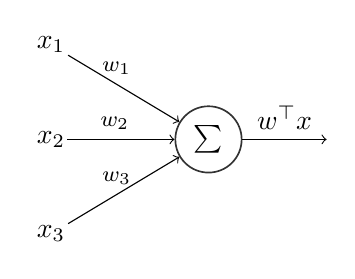
\begin{tikzpicture}
	\tikzstyle{neuron} = [circle,draw=black!80,semithick,minimum size=20pt]
	% input layer
	\foreach \i in {1,...,3}
		\node (input\i) at (0, -\i*1.2) {$x_\i$};
	% perceptron
	\node[neuron] (perceptron) at (2, -2*1.2) {$\sum$};
	% connections
	\foreach \i in {1,...,3}
		\draw[->, shorten <= -.1cm] (input\i) -- node[pos=.4,above]{\footnotesize{$w_\i$}} (perceptron);
	% output
	\draw[->] (perceptron) -- node[above]{$\bm{w}^{\top}\bm{x}$}(3.5, -2*1.2);
\end{tikzpicture}
	\end{center}
	\caption{An illustration of the perceptron model. In this example, the perceptron accepts three inputs $x_1, x_2, x_3$, has the parameters $w_1, w_2, w_3$, and computes $\hat{y} = \text{sign}(w_1x_1 + w_2x_2 + w_3x_3).$}
	\label{fig:perceptron}
\end{figure}

Perceptron models can be used to solve binary classification problems. In this scenario, we are given a set of $m$ training examples $\mathbb{X} = \{\bm{x}^{(1)}, \ldots, \bm{x}^{(m)}\}$ and their corresponding binary labels $\mathbb{Y}$, and wish to predict the most probable label for an unseen vector $\bm{x} \notin \mathbb{X}$.

For example, the vectors $\bm{x}^{(i)}$ might describe features of an email using a \emph{bag-of-words} representation. That is, we define a fixed vocabulary, and the $j$th entry in the vector $\bm{x}^{(i)}$ specifies how often the $j$th word of the vocabulary occurs in the particular email represented by $\bm{x}^{(i)}$. The corresponding label $y^{(i)} = 1$ then might signify that the email is a legitimate email, whereas a value of $y^{(i)} = -1$ might label the email as spam.

In the beginning, the weights are randomly initialized and the model thus makes arbitrary predictions. During the process of \emph{training} the perceptron, we iteratively adjust the weights in order to improve the prediction accuracy on the training set.

One common method of training is the perceptron learning algorithm proposed by \cite{Rosenblatt1958386}. Essentially, the algorithm iterates through the training data $\mathbb{X}$ and makes small adjustments to the weights if a particular training example $x^{(i)}$ is misclassified. For example, if the perceptron predicts $\hat{y} = 1$ and the actual label is $y^{(i)} = -1$, the weights are corrected in the negative direction. Since the perceptron learning algorithm is not directly applicable to neural networks, we will not discuss it further; a more in depth explanation can be found in \cite[Ch.\,8,\,pp.\,265-267]{DBLP:books/lib/Murphy12}.

A major shortcoming of the perceptron is that it can only learn to classify linearly separable data \cite{DBLP:books/daglib/0066902}. For example, the \textsc{xor} function, where 
\begin{equation}
\text{\textsc{xor}}(x) = 
\begin{cases} 0 & \text{if }x = [0,0] \lor x = [1,1] 
			\\1 & \text{if }x = [1,0] \lor x = [0,1],
\end{cases}
\end{equation}
cannot be learned with the perceptron. The discovery of these limitations has greatly reduced interest in the field of biological learning, until more sophisticated models, such as neural networks, were developed \cite[Ch.\,1,\,pp.\,12-18]{DBLP:books/daglib/0040158}.
	\end{center}
\end{figure}